\section{System Architecture}


\begin{figure}[ht]
    \centering
    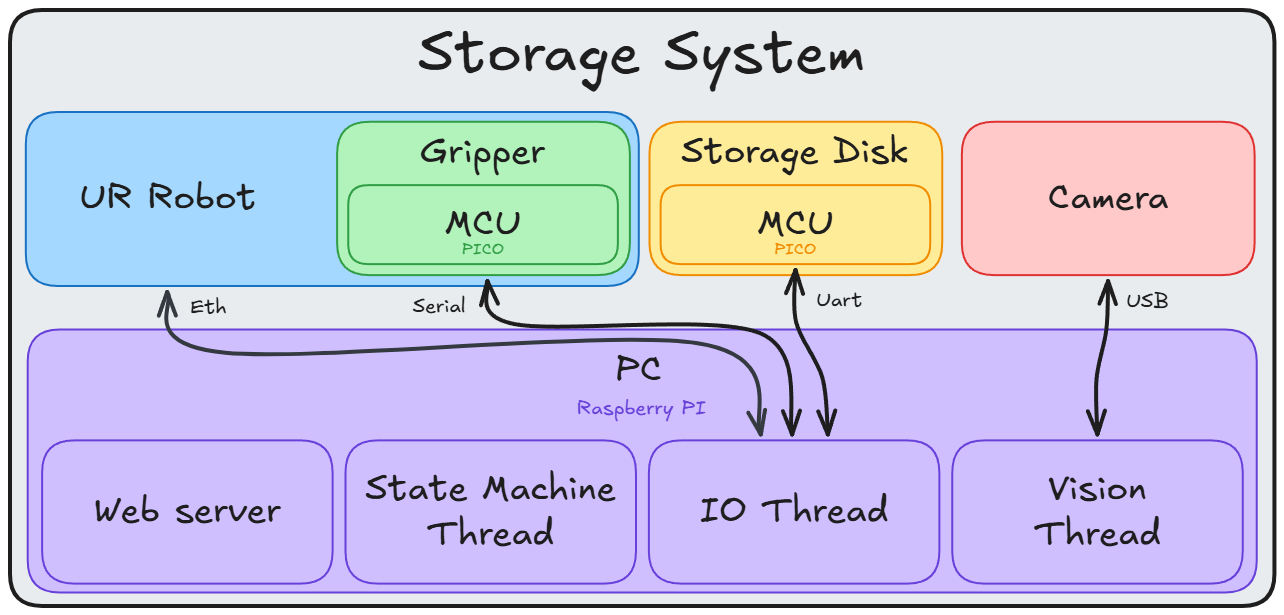
\includegraphics[width=0.8\textwidth]{figures/diagrams/SystemOverview.png}
    \caption{System overview}
    \label{fig:system-overview}
\end{figure}

As shown in \cref{fig:system-overview}, the system is built around a central control program running on the PC. The PC coordinates the robot arm, gripper, storage system and vision detection. The individual subsystems are kept separate so that each part can be developed and tested independently, while the central program controls the order in which actions are performed.

The robot arm is responsible for moving objects between the pickup area and the storage system. The gripper handles the physical grasping and releasing of objects. The storage system provides the physical storage positions, and the vision system supplies object position information to the rest of the system. The web interface gives the user a way to start, stop, and monitor the system.

This architecture keeps the high level coordination on the PC while the individual subsystems focus on their own tasks. The specific implementation of the robot control, vision processing, gripper software, and storage system is described in the following sections.

\subsection{PC software structure}
\label{sec:system-architecture}
The PC software is divided into a small number of threads. The \texttt{Orchestrator} contains the main state machine and controls the order of the workflow. It decides what should happen next, for example when the robot should move, when the gripper should close, and when the storage system should move to a specific position.

The physical communication is handled by an IO thread. This thread runs separately from the orchestrator and continuously updates the communication with the robot, gripper, and storage system. It is responsible for sending commands and reading responses, so the orchestrator does not have to block while waiting for hardware messages. Instead, the orchestrator can check whether a command is still running, has completed, has failed, or has timed out.

The vision system is handled by a separate vision thread. Image processing and object detection can take longer than the main control loop, so it is separated from the state machine. The vision thread can therefore work on locating objects while the rest of the program continues to run.

In addtion to these threads, a web server also runs it's own thread. It receives user commands such as start, stop, and reset, and it exposes the current system state, log messages, and selected measurement data. The web interface is shown in Appendix~\ref{app:web-interface}. These commands are forwarded to the orchestrator, which decides how they should affect the workflow.

\subsection{State machine}

\begin{figure}[H]
    \centering
    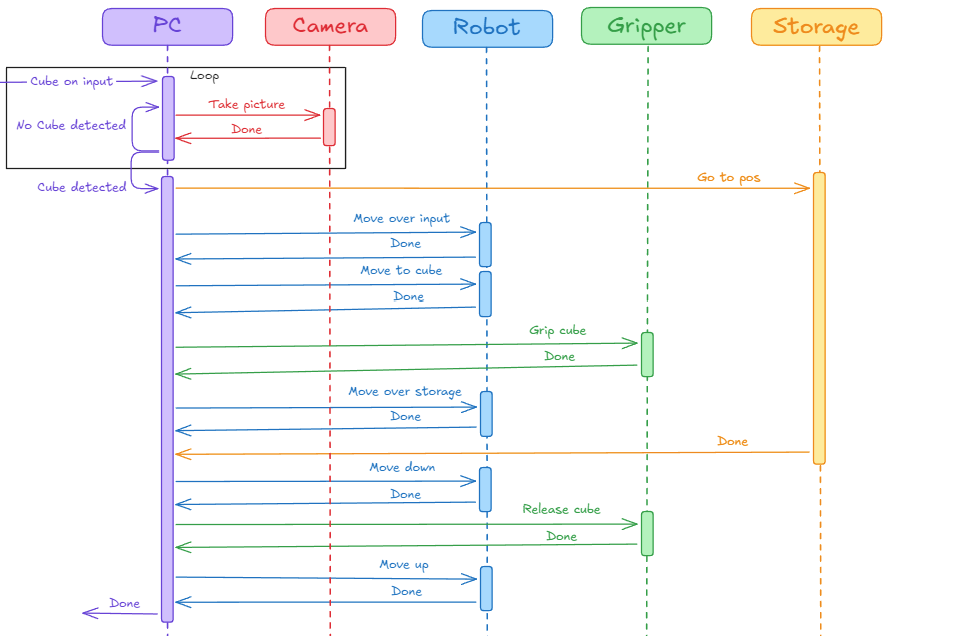
\includegraphics[width=1\textwidth]{figures/diagrams/StateMachineSequance.png}
    \caption{Machine sequence for a input-to-storage cycle}
    \label{fig:state-machine-sequence}
\end{figure}

The orchestrator is implemented as a state machine, as shown in \cref{fig:state-machine-sequence}. This means that the system is always in one defined state, and each state is responsible for a specific part of the workflow. The state machine makes the control flow explicit, which is important when several physical subsystems must work together in the correct order.

The system starts in the \texttt{Stopped} state. From here, a start command from the web interface moves the system to \texttt{Starting}. This state is used for startup actions such as preparing the robot and internal software state. When startup is finished, the system enters \texttt{Idle}, where it waits until an object is ready to be handled.

When the system begins an input-to-storage cycle, the state machine steps through the required actions one at a time. It selects a free storage slot, moves the robot towards the pickup area, closes the gripper, moves the object to the storage area, opens the gripper, and then returns to an idle state when the cycle is complete. Each physical action is treated as an operation that must finish before the next state is entered.

Stop and reset are handled as separate control paths. A stop command moves the system into \texttt{Stopping}, where active motion can be stopped before the system returns to \texttt{Stopped}. If an error occurs, such as a subsystem failing or timing out, the orchestrator moves to \texttt{Faulted}. From this state, a reset command clears the fault handling state and returns the system to a stopped condition.

This structure reduces the risk of starting a new action before the previous action has completed. It also makes faults easier to handle, because every command is evaluated from a known state and unexpected behaviour can be routed to the fault state instead of continuing the sequence.

